% Chapter 1: Introduction

\chapter{Introduction} % Chapter title

\label{ch:introduction} % For referencing the chapter elsewhere, use \autoref{ch:name}

Computer architectures have radically changed in the last 20 years with the introduction of thread-level parallelism in the form of multi-core architectures in almost all areas of computing:
from mobile computing to data centers and high-performance computing.
Furthermore, recently novel types of specialized architectures have been developed featuring large amounts of processing units for dealing with massively data-parallel workloads.
Parallelism and specialization are seen by many computer architects as two crucial answers for overcoming the challenges of increasing performance while at the same time increasing the energy efficiency~\cite{}.

% The development of mainstream programming languages and models have not kept pace with the hardware development.
These modern parallel processors are often still programmed with programming languages developed in the 1980's, like Java or C++, or even older languages like C (from the 1970's) or Fortran (from the 1950's).
These languages have a simplified view of the underlying hardware architecture often more or less directly resembling the Von Neuman architecture.
Multiple cores are programmed with libraries providing \emph{threads} where the programmer explicitly controls the computations on each core which execute the program in parallel.
This style of programming has turned out to be extremely difficult, as threads running concurrently on distinct cores can modify shared data which can lead to serious problems like deadlocks and non-determinism.
Even if the programmer develops a correct parallel implementation, optimizing this implementation for modern parallel processors is a challenging task even for experienced programmers.
Due to the lack of better programming systems, programmers are currently forced to develop hardware-specific implementations optimized towards a particular hardware architecture to achieve high performance.

This thesis describes our work to address these issues.
In the first part of the thesis we present a high-level programming model and its implementation which is designed to simplify the programming of modern parallel processors, especially systems comprising multiple Graphics processing units (\GPUs).
In the second part we discuss a system which generates high-performance code for different modern parallel processors, particularly a multi-core \CPU and two different types of \GPUs, from a single high-level program representation.
In the final part of the thesis we will outline how these two systems can be combined in the future to obtain a programming system which simplifies programming and achieves high-performance on different hardware architectures.

\noindent
We will start our discussion with an introduction on programming of modern parallel processors.
From this we will identify the two main challenges we tackle in this thesis:
the programmability challenge and the performance portability challenge.
We will then list our contributions before presenting the outline for the rest of the thesis.

%\section{On Programming Modern Parallel Processors}
\section{Modern Parallel Processors}

% processors become parallel
Traditionally, the performance of microprocessors has been mainly increased by boosting the clock frequency, optimize the execution flow, and improve caches~\cite{Sutter2005}.
This development has drastically changed around 10 years ago, as shown in \autoref{fig:cpuTrend}.
While the number of transistors continues to grow according to Moore's Law~\cite{Moore1998} the clock frequency and power consumption have hit a plateau around 2005.
\begin{figure}
  \centering
  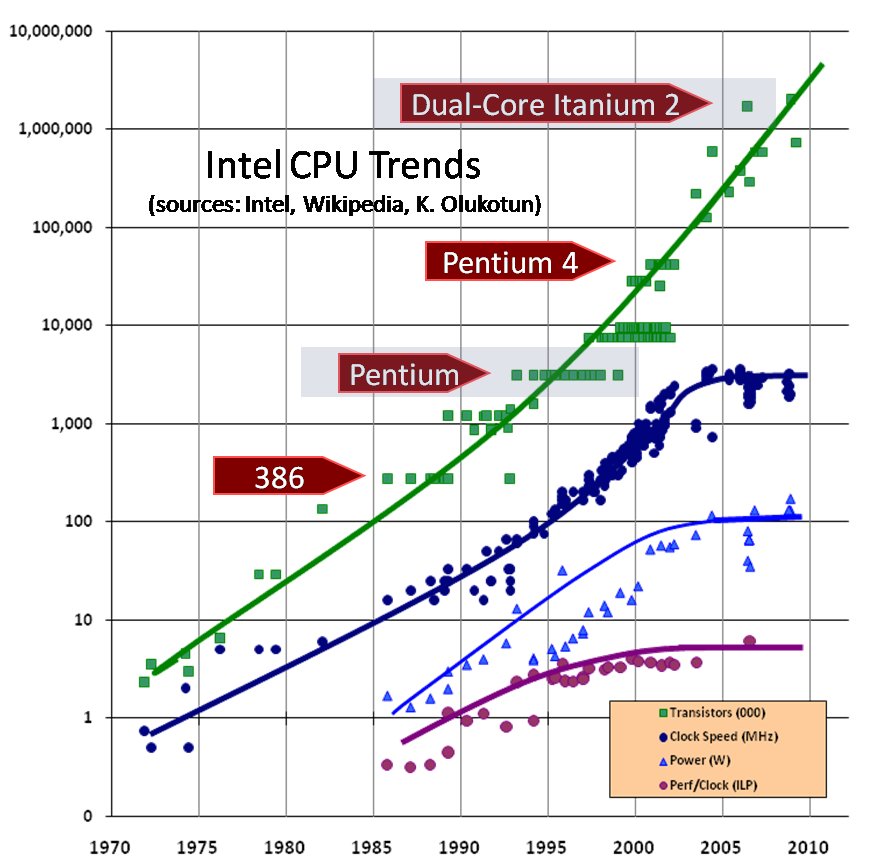
\includegraphics[width=.9\linewidth]{Figures/CPU.png}
  \caption{Development of Intel CPU over time. Inspired by~\cite{Sutter2005}}
  \label{fig:cpuTrend}
\end{figure} \todo{replace figure}
The reason for this lies in multiple physical effects, especially the physical limit of signal speed and increased heat development, which is mainly due to increased power consumption, both of which limit further increases of the clock frequency.
The predominant answer to this challenge has been the introduction of multiple distinct \emph{cores} which can operate concurrently.
% parallelism is now explicit to the programmer
Parallelism has been exploited in computer architectures for a long time at the bit level and the instruction level, but different than before with the introduction of multiple cores, this new \emph{thread-level parallelism} is explicit to the programmer.
This has profound effects on the design and development of software running on modern multi-core processors.
% programming with threads is a terrible idea
Most programming languages allow programmers to exploit multiple cores by the means of \emph{threads}.
A thread is a sequence of instructions defined by the programmer which can be scheduled by the runtime to be executed on a particular core.
Multiple threads can be executed concurrently and the programmer is responsible to use synchronization primitives, like locks or semaphores, for coordinating the execution of multiple threads.
Programming with threads is widely regarded as extremely difficult~\cite{} as subtle problems can arise which are hard to detect but can have severe consequences.
Nevertheless, threads are still the de-facto standard for programming multi-core \CPUs.

\bigskip

\noindent
% still moores law, no dennards scaling
% new hardware trend driven by energy efficiency, specialization, a.k.a heterogeneity, most prominent example: GPUs
While Moore's law still holds and transistor counts increase by further shrinking the transistor size, a related observation, known as Dennard scaling~\cite{DennardRiBaLe1974}, has broken down.
Dennard scaling suggested that power consumption is proportional with the area used for transistors on the chip.
Combined with Moore's law this meant, that the energy efficiency of processors doubled roughly every 18 month.
The primary reason for the breakdown of Dennard scaling around 2005 are physical effects appearing at the small scale of modern transistors, especially current leakage and increased heat development.
This has lead to architectures particular focused on their energy efficiency, the most prominent example of such architectures are modern Graphics Processing Units (\GPUs).
Originally developed for accelerating the rendering of complex graphics and 3D scenes, \GPUs architectures have been recently generalized to support more general purpose computations.
Some people refer to this development using the term general-purpose computing on graphics processing units (\GPGPU).

Technically \GPU architectures are multi-core architectures like modern multi-core \CPUs, but each individual core on a \GPU typically has dozens or hundreds of function units which can perform computations in parallel following the single instruction, multiple data (SIMD) principle.
These type of architectures are optimized towards a high throughput of computations, therefore, they focus on performing a large amount of operations in parallel and feature no, or only small, caches to prevent or mitigate latencies of the memory:
if a thread stalls wanting for the memory, another thread takes over and keeps the core busy.
For multi-core \CPUs switching between threads is more expensive, therefore, \CPUs are instead optimized to avoid long latencies when accessing the memory with a deep cache hierarchy and advanced architectural features, like long pipelines and out-of-order execution, all of which is designed to keep each core busy.

\section{The Programmability Challenge}

% programming on the CPU is a nightmare
Developing parallel programs for modern parallel processors is a challenging task.
The dominant approach for programming multi-core \CPUs is using multi-threading, \ie, explicitly managing the individual execution paths (called \emph{threads}) in a single program.
Threads communicate via a shared memory, where all threads have the possibility to modify any data item.
This fundamental principle gives the programmer much control over the interaction of the threads but greatly complicates the reasoning about the programs behavior.
The extensive and explicit control directly implies a very low level of abstraction, where the programmer deals with many details of the execution explicitly.
This makes the development of programs using threads complex and certain types of bugs more likely like deadlocks and data-races where the computed result depends on the order the threads are executed.
This ultimately leads to extensive problem during the development cycle as well as possible non-deterministic and undesirable behavior at runtime.

% not better on the GPU
Programming of \GPUs requires a different programming approach, as it is obviously infeasible to manage thousands of threads explicitly.
\CUDA~\cite{CUDAProgrammingGuide} and \OpenCL~\cite{OpenCL} are the two most popular approaches for programming \GPUs.
Both approaches are quite similar and require the programmer to write a function, called \emph{kernel}, which will be executed in parallel on the \GPU.
The kernel usually contains source code for identifying the thread executing the kernel which is used to coordinate on which data each thread operate on.
While this Single Program, Multiple Data (SPMD) programming model makes the management of threads feasible it does not address most problems associated with the low-level programming with threads.
For example, is explicit synchronization of threads still required and problems like deadlocks and race-conditions can still easily occur.
Furthermore, \GPU programming currently involves extensive boilerplate code to manage the execution on the \GPU, including the compilation of the kernel (in \OpenCL), transferring data to and from the \GPU, and launching the kernel by explicit specifying the number of threads to be started in parallel.

% There is a challenge: Programmability
All of this leads to our first central research question:
can we design a programming approach which significantly raise the level of abstraction and, thus, greatly simplify the development process of parallel applications, without sacrificing high-performance on multi-core \CPUs and \GPUs?
We will underpin the necessity to address this challenge with an extensive study of state-of-the-art \GPU programming using a concrete application example in \autoref{chapter:skelcl}.

In \autoref{part:skelcl} of this thesis, we will introduce, discuss, and evaluate a novel high-level programming model which attempts to address this \emph{challenge of programmability}.

\section{The Performance Portability Challenge}

% extracting performance is hard and not always predictable
Developing functional correct parallel applications for multi-core \CPUs or \GPUs is very challenging as we discussed in the preceding subsection.
Unfortunately, is the development of high-performing optimized applications even more demanding -- even for experienced programmers.
Applying optimizations often requires substantial restructuring of existing code.
Optimizations are often applied ad-hoc following certain ``rules of thumb'' derived from small-scale profiling and experiments as well as previously gained experience.
There exist no widely established approach for performing optimizations more systemically.
Especially, the performance implications of an assumed optimization is currently not predictable:
sometimes supposed optimizations leads to actual slowdowns in certain circumstances.

% compilers do a good job on low-level stuff, but fail for high-level optimizations
Modern optimizing compilers perform very sophisticated low-level optimizations, including various loop optimizations and optimization on data-flow analysis.
For all these type of optimizations, the compiler first has to recover parts of the high-level program semantics using analysis before applying the optimization.
As this analysis quickly becomes very complex compilers are ultimately limited in their optimization capabilities.
High-level optimizations which might restructure the entire source code are often out of the reach of low-level compiler optimizations and requires explicit and often extensive manual refactoring.
The state-of-the-art optimizing compilers simply are lacking the semantic high-level information necessary for performing these king of optimizations.

% optimizations are hardware-specific
Many optimizations exploit hardware-specific features and are, therefore, inherently not portable across hardware architectures.
As in current low-level programing model programmers encode these optimizations directly, programmers are forced with trade offs of either fully optimize their code for performance -- at the expense of code portability -- or implement a portable version -- at the expense of missing out on the highest performance possible.
Nowadays, programmers often choose a middle ground where introduce conditionals and branches in their code to select optimizations for the given hardware, while maintaining portability.
This, obviously, complicates the development process and decreases the maintainability of the software.

% There is a challenge: Performance Protability
This leads to our second central research question:
can we design a systematic approach where highly optimized, hardware-specific code is generated from a single high-level program representation?
We will confirm the lack of portability of performance in current state-of-the-art programming approaches using a study comparing optimizations on three different hardware architectures in \autoref{chapter:codeGeneration}.

In \autoref{part:codeGeneration} of this thesis, we will introduce, discuss, and evaluate a novel systematic code generation approach which attempts to address this \emph{challenge of performance portability}.


\section{Contributions of this Thesis}

This thesis makes the following four major contributions:

\subsection*{\hspace{2em}For Addressing the programmability challenge:}

\begin{description}
  \item[A High-level programming model for mutli-\GPU systems]\hfill\\[-1em]
    We present the design and implementation of our high-level programming model \SkelCL for programming multi-\GPU systems.
    \SkelCL offers three high-level features for simplified programming: container data types, algorithmic skeletons, and data distributions.
    We discuss our \Cpp library implementation of the \SkelCL programming model which is deeply integrated with \Cpp.
    Finally, we evaluate the level of abstraction and runtime performance of \SkelCL using a set of application studies.

  \item[Two novel algorithmic skeletons]\hfill\\[.25em]
    We introduce two novel algorithmic skeletons specialized towards \emph{allpairs} and \emph{stencil} computations.
    We present their formal definitions and discuss possible use cases in real world applications.
    For the allpairs skeleton we identify and formally define an optimization rule, which enables a more efficient implementation on \GPUs.
    We discuss and evaluate efficient implementations for both skeletons on a multi-\GPU system.
\end{description}

\subsection*{\hspace{2em}For Addressing the performance portability challenge:}

\begin{description}
  \item[A formal system for rewriting pattern-based programs]\hfill\\[-1em]
    We introduce a novel system comprising of set of high-level and low-level patterns along with a set of rewrite rules.
    The rewrite rules express high-level algorithmic and low-level optimization choices which can be systematically applied to transform a program expressed with our functional patterns.
    We proof the soundness of our approach by showing, that applying the rewrite rules does not change the program semantics.

  \item[A code generator offering performance portability]\hfill\\[.25em]
    Based on our formal rewrite system we present a novel code generator which generates from a single pattern-based program highly efficient \OpenCL code for three different hardware architectures:
    one multi-core \CPU and two different \GPUs.
    We discuss the design of our code generator and evaluate the performance of the generated \OpenCL code compared against highly optimized library code.
\end{description}

\section{Outline of this Thesis}
The remainder of this thesis is structured as follows.

\subsection*{Part I -- Introduction}

\paragraph{\autoref{chapter:background}} provides an introduction into the aspects of programming modern multi-core \CPUs and \GPUs.
We will start with the hardware where we mainly focus on \GPUs, discuss their architectures in detail, the state-of-the-art programming approaches, and optimization opportunities.
We will then shift our focus and discuss the algorithmic skeleton parallel programming model including its roots in functional programming.


\subsection*{Part II -- \SkelCL}

\paragraph{\autoref{chapter:skelcl}} addresses the programmability challenge identified in this chapter by introducing our novel \SkelCL high-level programming model targeted towards multi-\GPU systems and its implementation as a \Cpp library.
We will start by further motivating the need for high-level abstractions to simplify the software development process.
Then we present \SkelCL's three high-level features:
1) parallel container data types, 2) algorithmic skeletons, and 3) data distributions.
The combination of these features greatly simplifies the programming of multi-\GPU applications.
Finally, we will discuss the \SkelCL library implementation which is nicely integrated with \Cpp.

\paragraph{\autoref{chapter:skelcl-evaluation}} evaluates the \SkelCL programming model and library using multiple application studies.
We will start with discussing typical benchmark applications like the mandelbrot set computation and benchmarks from linear algebra.
We then continue with discussing more advanced applications from different areas, including image processing, medical imaging, physics, and bioinformatics.
We evaluate the increase of programmability and the performance of \SkelCL compared with implementations written in using the state-of-the-art \OpenCL programming approach.


\subsection*{Part III -- Code Generation using Patterns}

\paragraph{\autoref{ch:fifth}} addresses the performance portability challenge identified in this chapter by introducing a novel approach for generating highly optimized device-specific code from a single high-level program representation.
We will start the chapter with a study showing that optimizations in \OpenCL are not portable across different hardware architectures.
This emphasizes the motivation for performance portability to preserve maintainability while increase performance and efficiency at the same time.
Then we discuss the design of our code generation approach consisting of a set of parallel patterns combined with a set of rewrite rules.
The rewrite rules allow to rewrite pattern-based programs without changing their semantics which we will formally show.
Finally, we discuss how the rewrite rules can be systematically applied to optimize pattern-based programs for a particular hardware architecture.

\paragraph{\autoref{ch:sixth}} evaluates our code generation approach using a set of benchmark applications.
We evaluate the performance of the code generated using our approach and compare it against highly tuned library code on three different hardware architectures.

\subsection*{Part IV -- Summary \& Conclusions}

\paragraph{\autoref{ch:seventh}} summarizes Part II and Part II and describes their relation.
We will discuss how \SkelCL, presented in Part II, could be combined in the future with the code generator, presented in Part III, to obtain a system offering both high-level abstractions to simplify programming and high-performance on different hardware architectures.

\paragraph{\autoref{ch:eighth}} concludes the thesis by comparing against related work and discussing possible future extensions of our research.


%\section{Introduction}
%
%\from{HIPS begin}
%\subsection{HIPS}
%Modern \emph{Graphics Processing Units} (GPUs) provide large numbers of processing units and a high memory bandwidth.
%To enable \emph{General-Purpose Computation on GPU} (GPGPU), new programming models have been introduced, the two most popular approaches being CUDA and OpenCL~\cite{KirkHw2010,OpenCL}.
%While both programming models are similar, CUDA is a proprietary software developed by NVIDIA, whereas OpenCL is an open industry standard.
%
%Programming GPUs with OpenCL (and CUDA as well) still remains a difficult task because it is a low-level programming model:
%Data has to be transferred explicitly from the system's main memory (accessible by the CPU) to the GPU's memory and back.
%Moreover, memory allocation and deallocation also has to be explicitly controlled by the programmer.
%All this results in a lot of low-level boilerplate code in GPU programs.
%
%In this paper, we present \emph{SkelCL} --- a library which introduces an easy-to-use, high-level approach for GPU programming.
%SkelCL provides an abstract vector data type to perform data exchange between CPU and GPU implicitly.
%Pre-implemented communication and computation patterns (a.k.a. \emph{algorithmic skeletons}) based on this data type hide boilerplate code from the programmer inside the skeletons' implementations.
%Because SkelCL is based on OpenCL, it is not bound to a specific hardware and can be executed on any OpenCL-capable device.
%\from{HIPS end}
%
%\from{ASHES begin}
%\subsection{ASHES}
%
%The two popular programming approaches for systems with \emph{Graphics Processing Units} (GPUs) --- CUDA and OpenCL~\cite{OpenCL,CUDAProgrammingGuide,KirkHw2010} --- work at a low level of abstraction.
%They require the programmer to explicitly manage the GPU's memory, including data allocations and transfers to/from the system's main memory.
%This leads to long, complex and, therefore, error-prone code.
%The emerging multi-GPU systems are particularly challenging for the application developer:
%they additionally require explicit data exchanges between individual GPUs, including low-level pointer arithmetics and offset calculations, as well as an adaption of algorithms for execution on multiple GPUs.
%
%In this paper, we introduce SkelCL --- a library for high-level GPU programming.
%SkelCL comprises two major abstraction mechanisms: a set of algorithmic skeletons~\cite{Cole1991} and an abstract vector data type.
%Skeletons offer several frequently used pre-implemented patterns of parallel communication and computation to the application developer.
%The vector data type enables implicit data transfers between the system's main memory and GPUs.
%Using these abstractions, SkelCL frees the programmer from writing low-level and error-prone boilerplate code when programming multi-GPU systems, and still provides all useful features of the OpenCL standard.
%
%The focus of this paper, as compared to our introductory article~\cite{SteuwerKeGo2011}, is the set of specific features and mechanisms of SkelCL for programming multi-GPU systems on a high level of abstraction.
%We describe how SkelCL implements skeletons on multi-GPU systems and show how SkelCL's concept of \emph{data distribution} frees the user from low-level memory management, without sacrificing performance in real-world applications that use multiple GPUs.
%
%\from{ASHES end}
%
%\from{Paraphrase begin}
%\subsection{Paraphrase}
%Application programming for GPUs (Graphics Processing Units) is complex and error-prone.
%The popular programming models for systems with GPUs -- CUDA and OpenCL~\cite{CUDAProgrammingGuide,KirkHw2010,OpenCL} -- require the programmer to explicitly manage GPU's memory, including (de)allocations and data transfers to/from the system's main memory.
%This leads to lengthy, low-level, complex and thus error-prone code.
%For emerging systems with multiple GPUs, CUDA and OpenCL additionally require an explicit implementation of data exchange between GPUs and separate management of each GPU.
%This includes low-level pointer arithmetics and offset calculations, as well as explicit program execution on each GPU.
%Neither CUDA nor OpenCL offer specific support for such systems, which makes their programming even more complex.
%
%In this paper, we first briefly describe our SkelCL library~\cite{SteuwerKeGo2011} for high-level single- and multi-GPU computing.
%It offer pre-implemented recurring computation patterns (\emph{skeletons}) for simplified GPU programming.
%In addition, the application developer is freed from memory management, which is done implicitly in SkelCL.
%
%As a specific contribution of the paper, we add a new two-dimensional data type and an additional skeleton to SkelCL.
%The \emph{matrix} data type complements the one-dimensional vector data type for working with two-dimensional data, e.g., matrices or images.
%The new \emph{MapOverlap} skeleton executes a given function on every element of the input data, using also the values of its neighboring elements.
%Another novel contribution of this paper is the data distribution mechanism for simplifying two-dimensional data processing on systems with multiple GPUs.
%Finally, we present an application case study using the matrix data type and the MapOverlap skeleton -- Sobel edge detection for 2D images -- and report experimental results using SkelCL.
%
%The paper is organized as follows.
%First we briefly introduce the basics of SkelCL in Section~\ref{sec:skelcl} using our previous work~\cite{SteuwerKeGo2011}.
%The MapOverlap skeleton is then introduces in Section~\ref{sec:skelcl:mapoverlap} and the matrix data type in Section~\ref{sec:skelcl:matrix}.
%In Section~\ref{sec:application_study} we demonstrate how both are used together to implement an application from the area of image processing: the Sobel edge detection.
%We report experimental results and we evaluate performance and usability of our approach.
%Section~\ref{sec:conclusion} concludes the paper and compares our approach to related work.
%\from{Paraphrase end}
%
%
%\from{ICCS begin}
%\subsection{ICCS}
%Modern high-performance computer systems increasingly employ \emph{Graphics Processing Units} (GPUs) and other accelerators.
%The state-of-the-art application development for systems with GPUs is cumbersome and error-prone, because GPUs are programmed using relatively low-level models like CUDA~\cite{CUDAProgrammingGuide} or OpenCL~\cite{OpenCL}.
%These programming approaches require the programmer to explicitly manage GPU's memory (including memory (de)allocations, and data transfers to/from the system's main memory), and to explicitly specify parallelism in the computation.
%This leads to lengthy, low-level, complex and thus error-prone code.
%For multi-GPU systems, programming with CUDA and OpenCL is even more complex, as both approaches require an explicit implementation of data exchange between GPUs, as well as separate management of each GPU, including low-level pointer arithmetics and offset calculations.
%
%In this paper, we describe the SkelCL (Skeleton Computing Language) -- a high-level programming model for parallel systems with multiple GPUs.
%The model is based on the OpenCL standard and extends it with three novel, high-level mechanisms:
%\begin{itemize}
%  \item[1)] \emph{parallel skeletons}: pre-implemented high-level patterns of parallel computation and communication which can be customized and combined to express application-specific parallelism;
%  \item[2)] \emph{parallel container data types}: collections of data (e.\,g., vectors and matrices) that are managed automatically across all GPUs in the system;
%  \item[3)] \emph{data (re)distributions}: an automatic mechanism for describing data distributions and re-distributions among the GPUs of the target system.
%\end{itemize}
%
%The paper describes how the SkelCL model is used for programming a sample real-world application from the area of medical imaging, and how the model is implemented as the SkelCL programming library, using C++.
%Our focus is on programming methodology;
%therefore, we motivate our work using one typical imaging application and then study it in great detail throughout the paper.
%\from{ICCS end}
%
%\from{HLPP begin}
%\subsection{HLPP}
%Algorithmic skeletons enable application developers to program parallel systems at a high level of abstraction~\cite{Cole1991}.
%Skeletons abstract recurring patterns of parallel programming and provide efficient parallel implementations for these patterns.
%The application developer uses skeletons by providing application-specific code (so-called customizing function) which customizes the skeletons' behavior.
%Skeletons thus allow the application developer to focus on the structure of the algorithms, rather than on their implementation details.
%
%We develop SkelCL~\cite{SteuwerKeGo2012} -- a skeleton library for programming modern many-core architectures, especially systems with Graphics Processing Units (GPUs).
%Programming these systems using the current low-level approaches like CUDA~\cite{CUDAProgrammingGuide} and OpenCL~\cite{OpenCL} is challenging: parallelism has to be expressed explicitly by defining and executing parallel \emph{kernels}, and memory management is cumbersome, as data has to be moved manually to and from the GPU memory.
%By providing skeletons on container data types, SkelCL alleviates programming of systems with GPUs:
%parallelism is expressed implicitly, using skeletons, and memory management is performed automatically by the SkelCL implementation built on top of OpenCL.
%The especially tricky programming of multi-GPU systems is greatly simplified by SkelCL's data distribution mechanism which automatically moves data between multiple GPUs.
%
%In this paper, we aim at \emph{allpairs computations} which occur in a variety of applications, ranging from matrix multiplication and pairwise Manhattan distance computations in bioinformatics~\cite{ChangDeQuRo2009} to N-Body simulations in physics~\cite{AroraShVu2009}.
%These applications share a common computational pattern:
%for two sets of entities, the same computation is performed independently for all pairs in which entities from the first set are combined with entities from the second set.
%Previous work discussed specific allpairs applications and their parallel implementations on multi-core CPUs~\cite{AroraShVu2009}, the Cell processor~\cite{WirawanSK09}, and GPUs~\cite{ChangDeQuRo2009,SarjeAl2013};
%it demonstrated that developing well-performing implementations for allpairs is challenging, especially on GPU systems, as it requires exploiting their complex memory hierarchy and assumes a deep knowledge of the target hardware architecture.
%
%The contributions and structure of this paper are as follows.
%To enable application developers to efficiently use the allpairs computational pattern, we formally define the allpairs skeleton and provide its generic parallel implementation in OpenCL (Section~\ref{sec:allpairs_skeleton}).
%We optimize the use of the GPU memory hierarchy by implementing a specialized version of the allpairs skeleton with a customizing function that follows a certain memory access pattern (Section~\ref{sec:opt_allpairs_skeleton}).
%We show that our implementations can be used for single- and multi-GPU systems (Section~\ref{sec:multi_gpu}).
%We evaluate the runtime performance and the programming effort of the allpairs skeleton within the SkelCL library, using matrix multiplication as application study (Section~\ref{sec:experiments}).
%We discuss related work and conclude in Section~\ref{sec:conclusion}.
%\from{HLPP end}
%
%\from{PaCT begin}
%\subsection{PaCT}
%Modern high-performance computer systems become increasingly heterogeneous as they comprise in addition to multi-core processors, also \emph{Graphics Processing Units} (GPUs), Cell processors, FPGA, and other accelerating devices, usually called \emph{accelerators}.
%The state-of-the-art application programming for systems with GPUs is cumbersome and error-prone, because GPUs are programmed using explicit, low-level programming approaches like CUDA~\cite{CUDAProgrammingGuide} or OpenCL~\cite{OpenCL}.
%These approaches require the programmer to explicitly manage GPU's memory (including memory (de)allocations, and data transfers to/from the system's main memory), and explicitly specify parallelism in the computation.
%This leads to lengthy, low-level, complicated and, thus, error-prone code.
%For multi-GPU systems, programming with CUDA and OpenCL is even more complex, as both approaches require an explicit implementation of data exchange between the GPUs, as well as disjoint management of each GPU, including low-level pointer arithmetics and offset calculations.
%
%In this paper, we describe the \emph{SkelCL} (Skeleton Computing Language) -- our high-level programming approach for parallel systems with multiple GPUs.
%The SkelCL programming model is based on the OpenCL standard and enhances it with three high-level mechanisms:
%\begin{itemize}
%  \item[1)] \emph{parallel container data types}: collections of data (in particular, vectors and matrices) that are managed automatically on all GPUs in the system;
%  \item[2)] \emph{data (re)distributions}: an automatic mechanism for specifying in the application program suitable data distributions and re-distributions among the GPUs of the target system:
%  \item[3)] \emph{parallel skeletons}: pre-implemented high-level patterns of parallel computation and communication which can be customized to express application-specific parallelism, and combined to a large high-level code.
%\end{itemize}
%The structure of the paper is as follows.
%In Section \ref{sec:requirements} we formulate the requirements to a high-level programming approach for GPU systems, following from the analysis of compute-intensive applications.
%Section \ref{sec:skelcl} describes in detail our SkelCL approach.
%In Section \ref{sec:studies} we report experimental evaluation of our approach regarding both programming effort and performance.
%We compare to related work and conclude in Section in Section \ref{sec:conclusion}.
%\from{PaCT end}
%
%\from{HiStencils begin}
%\subsection{HiStencils}
%Stencil computations play an important role in a number of different application domains including time-intensive scientific simulations, image processing and others.
%Modern manycore architectures with Graphics Processing Units (GPUs) and other accelerators provide potentially tremendous computing power for challenging applications including stencil computations.
%
%However, the current programming approaches for manycore architectures are low level, the most popular examples being OpenCL~\cite{OpenCL} and CUDA~\cite{CUDAProgrammingGuide}.
%These approaches require the programmer to explicitly manage GPU's memory (including memory (de)allocations and data transfers to/from the system's main memory) and explicitly specify parallelism in the computation.
%This leads to lengthy, low-level, complicated and, thus, error-prone code.
%For multi-GPU systems, programming with CUDA and OpenCL is even more complex, as both approaches require an explicit implementation of data exchange between the GPUs, as well as disjoint management of each GPU, including low-level pointer arithmetics and offset calculations.
%When implementing stencil computations, additional challenges arise, like handling out-of-bound memory accesses and achieving high performance by making efficient use of the fast but small local GPU memory.
%
%In this paper, we present our SkelCL~\cite{SteuwerGo2013a} approach to high-level, manycore programming, and we describe how it simplifies stencil programming and achieves competitive performance on multi-GPU systems.
%SkelCL extends the OpenCL standard by three high-level mechanisms:
%\begin{itemize}
%  \item[1)] computations are easily expressed using pre-implemented parallel patterns (a.k.a. \emph{skeletons});
%  \item[2)] memory management is simplified using \emph{container data types} for vectors and matrices;
%  \item[3)] data movement in multi-GPU systems are handled automatically by SkelCL's \emph{(re)distribution mechanism}.
%\end{itemize}
%
%For stencil computations, we extend SkelCL with two specialized skeletons: MapOverlap for simple stencil computations, and Stencil for more complex, in particular iterative, stencil computations.
%\from{HiStencils end}
%
%\from{PACT begin}
%\subsection{PACT}
%Computing systems have now become extremely complex and diversified in part due to the recent emergence of GPUs (Graphic Processing Units) for general purpose computation.
%The drawback of such systems is the extreme difficulty of extracting performance, requiring a deep understanding of the hardware.
%This means that software written and tuned for today systems needs to be adapted frequently to keep pace with ever changing hardware.
%
%Over the years, a wide range of languages, language extensions and frameworks have emerged for programming GPUs and other parallel devices.
%The two most common low-level languages are CUDA and OpenCL, both directly exposing hardware features.
%Directive based languages such as Cilk~\cite{BlumofeJKLRZ95}, Open\-ACC~\cite{ReyesLFS12} and OpenMP~\cite{LeeME09} or libraries like Intel TBB~\cite{Reinders07} have been proposed to reduce the complexity of developing code for multicore CPUs and GPUs.
%These approaches simplify writing applications, but still require the programmer to tune the application for a particular hardware device.
%As a result, \emph{performance portability} remains elusive; code optimized for one device might only achieve a fraction of the performance on a different device, as shown by our results.
%
%Several high-level programming models have been proposed to address this issue.
%Petabricks~\cite{PhothilimthanaARA13} allows the programmer to express different algorithm implementations and automatically picks the best one using auto-tuning.
%It can also automatically identify and translate algorithms that are suitable for GPU execution.
%Higher-level dataflow programming language such as StreamIt~\cite{HormatiSWMM11} or LiquidMetal~\cite{DubachCRBF12} have been designed with a similar goal in mind.
%Both languages use dedicated backend compiler for different hardware targets such as GPUs.
%A recent trend is the adoption of a more functional programming approach.
%For instance, Nvidia's NOVA~\cite{CollinsGGLS14} language exposes algorithmic patterns such as \pat{map} or \pat{reduce} as function primitives recognized by the backend compiler.
%While definitively a step in the right direction, all these approaches still rely on hard-coded device-specific implementations or heuristics.
%When hardware changes occur, the backend compiler has to be re-tuned or re-engineered.% in the presence of a new hardware features.
%
%The root of the problem lies in the gap in the system stack between high-level algorithmic concepts on the one hand and low-level hardware paradigms on the other.
%To bridge this gap, we propose a novel approach based on algorithmic pattern and low-level hardware pattern composition and a set of rewrite rules.
%While similar in spirit to Spiral~\cite{PueschelMJPVSXFGVCJR2005}, our approach relies on fine grain hardware patterns representing CPUs and GPUs hardware features exposed by the OpenCL programming model.
%The rewrite rules are used to automatically derive semantically equivalent low-level expressions from high-level algorithm expressions written by the programmer.
%Once derived, we automatically generate high performance OpenCL code based on these expressions.
%This makes the code generator very simple since all decisions related to optimizations are handled during the automatic rewriting process.
%
%The power of our approach lies in the rewrite rules, written once by an expert system designer.
%These rules encode the different algorithmic choices and low-level optimizations.
%The rewrite rules play the dual role of enabling the composition of algorithmic patterns and enabling the lowering of these patterns onto the low-level hardware paradigms.
%This results in a clear separation of concerns between high-level algorithmic patterns and low-level hardware paradigms.
%Producing high performance code is achieved by automatically searching the implementation space defined by applying the rewrite rules.
%
%This paper demonstrates the applicability of our approach on a map-reduce style of patterns.
%Map and reduce are common performance critical programming patterns used as building blocks for many algorithms~\cite{AsanovicBoCaGeHuKePaPlShWiYe2006}.
%We compare our approach with highly-tuned linear algebra functions extracted from the state-of-the-art libraries and with larger type of benchmarks such as BlackScholes.
%Our performance is competitive with highly-tuned implementations of the BLAS linear algebra library such as Nvidia GPU CUBLAS~\cite{cuBLAS}, AMD GPU clBLAS~\cite{clBLAS} and ATLAS~\cite{WhaleyD98} on the CPU.
%Interestingly, this is achieved without specializing the compiler towards a specific hardware target.
%Instead, we automatically build and search the implementation space by expressing our high-level algorithmic patterns as a composition of low-level hardware patterns.
%Our paper makes the following key contributions:
%\vspace{0.2em}
%\begin{itemize}
%  \item design of \textbf{low-level hardware patterns} that represents the OpenCL programming model; \vspace{0pt}
%  \item develop a powerful set of \textbf{algorithmic and low-level rules} that expresses algorithmic and optimization choices; \vspace{0pt}
%  \item demonstrate that \textbf{performance portability} can be achieved via an automated search of possible implementations, leading to performance in par with the best hand-tuned versions. \vspace{0pt}
%\end{itemize}
%\from{PACT end}
%
%
%% \section{Introduction} end
%
%
%\from{PaCT begin}
%\section{Requirements to a High-Level Programming Model (PaCT)}
%To simplify programming for a system with multiple GPUs, the following high-level abstraction are desirable:
%
%\paragraph{Parallel container data types}
%Compute-intensive applications typically operate on a (possibly big) set of data items.
%Managing memory hierarchy of multi-GPU systems explicitly is complex and error-prone because low-level details, like offset calculations, have to be programmed manually.
%A high-level programming model should be able to make collections of data automatically accessible to all GPUs in the target system and it should provide an easy-to-use interface for the application developer.
%
%\paragraph{Distribution and redistribution mechanisms}
%To achieve scalability of applications on systems comprising multiple GPUs, it is crucial to decide how the application's data are distributed across all available GPUs.
%Applications often require different distributions for their computational steps.
%Distributing and re-distributing data between GPUs in OpenCL is cumbersome because data transfers have to be managed manually and performed via the CPU.
%Therefore, it is important for a high-level programming model to allow both for describing the data distribution and for changing the distribution at runtime, such that the system takes care of the necessary data movements.
%
%\paragraph{Recurring patterns of parallelism}
%While the concrete operations performed in an application are (of course) application-specific, the general structure of parallelization often follows some common parallel patterns that are reused in different applications.
%For example, operations can be performed for every entry of an input vector, which is a well-known pattern of data-parallel programming, or two vectors are combined element-wise into an output vector, which is again a common pattern of parallelism.
%It would be, therefore, desirable to express the high-level structure of an application using pre-defined common patterns, rather than describing the parallelism explicitly in much detail.
%\from{PaCT end}

